\documentclass[11pt]{article}

\usepackage[margin=1.5cm]{geometry}

%--------------------------------------
%\usepackage[russian]{babel}
\usepackage{fontspec}

\setmainfont[Ligatures=TeX]{Montserrat}
\setmonofont[Ligatures=TeX]{Courier New}
%--------------------------------------

\usepackage{fancyvrb}
\usepackage{fvextra}
\DefineShortVerb{\|}
\usepackage{graphicx}
\usepackage{csvsimple}
\usepackage{longtable}

\begin{document}

    \begin{center}
    \vspace*{1cm}
    \Huge
    Алгоритми та структури даних\\
    \textbf{Лабораторна робота 2: Алгоритми сортування}\\
    \Large
    Варіант 6\\
    \vspace{0.5cm}
    Протокол\\
    \vspace{1.5cm}
    \textbf{Михайло Корешков}\\
    ФІ-81
    \vfill
    Фізико-Технічний Інститут\\
    НТУУ "КПІ ім. Ігоря Сікорського"\\
    2020
\end{center}
\newpage

    \renewcommand*\contentsname{Зміст}
    \tableofcontents
    \newpage


    \section{Структура}
    \VerbatimInput[frame=single, framesep=2mm,breaklines=true]{structure.txt}


    \section{Проектні рішення}

    \subsection{Алгоритм швидкого сортування}
    Я вирішив обрати не-рекурсивний підход із використанням додаткового стеку "задач" -
    вектор кортежів типу (Int, Int), які містять індекси початку та кінця підмасиву,
    який потрібно відсортувати наступним.
    Перше, що відбувається у основному циклі - зі стеку виймається задача.
    Цикл продовжується доки стек задач не пустий.


    \section{Аналіз швидкодії}
    Графіки залежності кількості операцій від розміру масива.
    Масштаб log2-log2.
    Окремо для парних та непарних N.

    \section{Висновки}
    Основний висновок - Quicksort значно швидший за Bubblesort, але тільки починаючи з деякого значення N.
    Для N=1000 кількість обмінів Quicksort у більш ніж 1000 разів менша за таку в Bubblesort.

    \subsection{Вихідні дані порівняння}
    \VerbatimInput[breaklines=true,breakanywhere=true,numbers=left]{../src/mk-sorting-report.csv}

    \section{Графіки}

    \begin{figure}[H]
        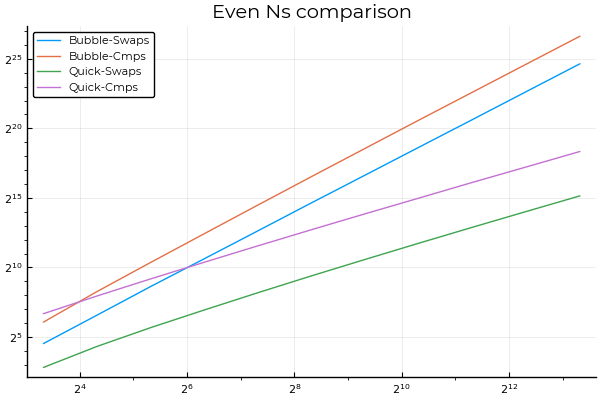
\includegraphics[width=0.8\textwidth]{../out/even.png}
        \caption{Парні N}
    \end{figure}

    \begin{figure}[H]
        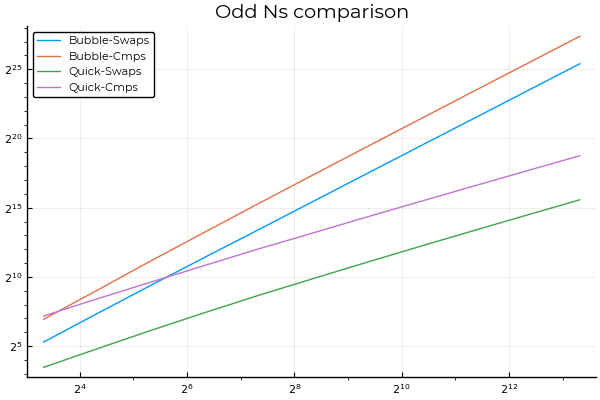
\includegraphics[width=0.8\textwidth]{../out/odd.png}
        \caption{Непарні N}
    \end{figure}

    \section{Код}
    \VerbatimInput[breaklines=true,breakanywhere=true,numbers=left]{../src/sorting.jl}

\end{document}